%%%%%%%%%%%%%%%%%%%%%%%%%%%%%%%%%%%%%%%%%%%%%%%%%%%%%%%%%%%%%%%%%%%%%%
% LaTeX Example: Project Report
%
% Source: http://www.howtotex.com
%
% Feel free to distribute this example, but please keep the referral
% to howtotex.com
% Date: March 2011 
% 
%%%%%%%%%%%%%%%%%%%%%%%%%%%%%%%%%%%%%%%%%%%%%%%%%%%%%%%%%%%%%%%%%%%%%%
% How to use writeLaTeX: 
%
% You edit the source code here on the left, and the preview on the
% right shows you the result within a few seconds.
%
% Bookmark this page and share the URL with your co-authors. They can
% edit at the same time!
%
% You can upload figures, bibliographies, custom classes and
% styles using the files menu.
%
% If you're new to LaTeX, the wikibook is a great place to start:
% http://en.wikibooks.org/wiki/LaTeX
%
%%%%%%%%%%%%%%%%%%%%%%%%%%%%%%%%%%%%%%%%%%%%%%%%%%%%%%%%%%%%%%%%%%%%%%
% Edit the title below to update the display in My Documents
%\title{Project Report}
%
%%% Preamble
\documentclass[paper=a4, fontsize=11pt]{scrartcl}
\usepackage[T1]{fontenc}
\usepackage{fourier}

\usepackage[english]{babel}															% English language/hyphenation
\usepackage[protrusion=true,expansion=true]{microtype}	
\usepackage{amsmath,amsfonts,amsthm} % Math packages
\usepackage[pdftex]{graphicx}	
\usepackage{url}
\usepackage{lipsum}


%%% Custom sectioning
\usepackage{sectsty}
\allsectionsfont{\raggedright \bfseries\scshape}


%%% Custom headers/footers (fancyhdr package)
\usepackage{fancyhdr}
\pagestyle{fancyplain}
\fancyhead{}											% No page header
\fancyfoot[L]{}											% Empty 
\fancyfoot[C]{}											% Empty
\fancyfoot[R]{\thepage}									% Pagenumbering
\renewcommand{\headrulewidth}{0pt}			% Remove header underlines
\renewcommand{\footrulewidth}{0pt}				% Remove footer underlines
\setlength{\headheight}{13.6pt}


%%% Equation and float numbering
\numberwithin{equation}{section}		% Equationnumbering: section.eq#
\numberwithin{figure}{section}			% Figurenumbering: section.fig#
\numberwithin{table}{section}				% Tablenumbering: section.tab#


%%% Maketitle metadata
\newcommand{\horrule}[1]{\rule{\linewidth}{#1}} 	% Horizontal rule
\renewcommand{\baselinestretch}{1.5}


\title{
		%\vspace{-1in} 	
		\usefont{OT1}{bch}{b}{n}
		\normalfont \normalsize \textsc{Institute of Scientific Computing\\Technische Universität Dresden\\
		Modeling and Simulation Seminar \\
		Group-Shape Optimization} \\ [25pt]
		\horrule{0.5pt} \\[0.4cm]
		\huge Modeling of Thin membranes \\ 
		\horrule{2pt} \\[0.5cm]
}
\author{
		\normalfont 								\normalsize
        Anurag Trivedi, anurag.trivedi@mailbox.tu-dresden.de \\[-3pt] \normalsize
        Mohammed Parvez, Parvez.Mohammed@mailbox.tu-dresden.de\\[-3pt]		\normalsize
        \today
}
\date{}


%%% Begin document
\begin{document}
\vspace{5mm}

\maketitle
\section{Abstract}

This work aims to show that a simple, structured, and efficient shape optimization framework can be written by using finite element software AMDiS. This is illustrated by the implementation of a classical technique called geometrical optimization for such type of problem. we modeled theoretical and computational work for 2D Problems to develop robust technique. Our computational Result is very useful for engineers or researchers.
\section{Introduction}
The goal is to Optimize the shape of a thin Membrane subjected to certain load and boundary conditions. We explore Quadrature with the finite element method. In PDE-constrained optimization, we have two choices for discretization whether to discretize-then-optimize or optimize-then-discretize. we have chosen a discretize-then-optimize approach. because most optimization problems are naturally self ad-joint and by this choice, we can avoid non-symmetry due to discretization that can arise with the optimize-then-discretize approach. So that we are able to use the iterative method is the projection Gradient method. However, it would be impractical to write the code for the entire finite element method from scratch. This project aims to use AMDiS, open-source software for FEM, to deal with the nuances of FEM such as mesh generation, calculation of numerical solutions of PDEs, etc then write simple shape optimization routines.

\subsection{Shape Optimization of Structure}

The problem of Shape Optimization of structures is defined by three ingredients
\begin{description} 
 \item
1. A Mathematical model to evaluate the mechanical behavior of a structure.
 \item
2. an Objective function which has to be minimized or maximized, or sometimes several objectives (also called cost-functions or criteria).
 \item
3. Set of admissible thicknesses which precisely defines the optimization variables, including possible constraints.


\end{description}

\subsubsection{Mathematical Model}

In our mathematical model, we consider our membrane to be fixed at the boundaries and subject to some vertical force $f: \Omega \rightarrow R $. Due to very small deformations, the membrane can be modeled by its vertical displacement $u: \Omega \rightarrow R $, the solution to PDE. 


\begin{align} 
	\begin{split}
	-div(h \nabla u)	= f in $\Omega$\\
					u =0 on \partial $\Omega$\\
					\end{split}					
\end{align}


	
	
The thickness h is our optimization variable. It is bounded by some given minimum and maximum values:
\begin{center}



$0< h_{min} \leq h(x) \leq h_{max} < \infty$
\end{center}

\subsubsection{Objective function}
The optimization of the structure can be linked to some mechanical properties.
\begin{center}



$J(h) = \int_{\Omega} j(u) dx  $
\end{center} 

It could be the optimization to achieve a target displacement
\begin{center}



$j(u) =  |u - u_{0}|^2$
\end{center} 

It could also be to minimize the max stress-induced.

\begin{center}



$J(h) = sup_{x \in \Omega} |\sigma (x)|$
\end{center} 
We, however, in this project are optimizing for compliance(-rigidity)
\begin{center}



$j(u) = fu$
\end{center} 
\subsubsection{Set of admissible thicknesses}

{\bf{Volume constraint}}


Many structural optimization problems feature a volume constraint on the admissible open sets.
\begin{center}



$U_{ad} = \{h \in L^{\infty}(\Omega): $0< h_{min} \leq h(x) \leq h_{max} < \infty$ in $\Omega$, \int_{\Omega} h(x)dx = h_{0}|\Omega| \} $
\end{center}
In this project, we have considered our thickness function to be piece-wise constant on a coarse grid other than the discretization grid that is used in the FEM formulation by AMDiS.
\begin{center}


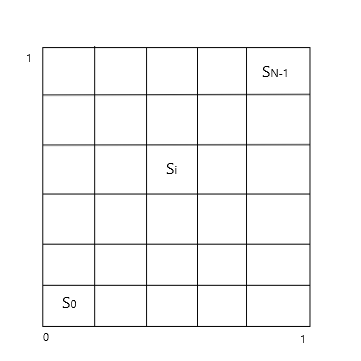
\includegraphics[scale=0.7]{grid.png}\\
Fig 1-Grid
\end{center}


Hence our admissible open set is
\begin{center}
$U_{ad} & =  \{ h(x)= \sum^{N-1}_{i=0} h_{i} I_{s_{i}}(x); 0 < 0.1 \leq h_{i}(x) \leq 5,  \sum^{N-1}_{i=0} h_{i}(x)  = N \}$
\end{center}
Where $N$ is the total number of grid cells and $I_{s{i}}$ is the indicator function for $i'th$ rectangular grid cell. 

This constraint is imposed by introducing the Lagrange multiplier $'l'$ in the formulation. Hence, the descent direction is now computed from the shape derivative of the Lagrangian

\begin{center}



$J'(\Omega)+ l V'(\Omega)$
\end{center}
where $V(\Omega)$ is volume of $\Omega$, $ 'l' $ is Lagrange multiplier.\\
The Lagrange multiplier is updated in each iteration by 


\begin{center}



$ l = 2(\frac{\int_{\Omega}  \tilde{h^{n+1}}  dx -1 }{N})$
\end{center}
Where $\tilde{h_{n}}$ is the thickness that is obtained from gradient descent without projection(see section 3.1)


\section{Numerical algorithm}
We are presented numerical schemes for solving these kinds of the minimization problem. The iteration schemes starting from giving initial value $h^{0}$ we construct a sequence $(h^{n})_{n \in N}$, which can be shown to converge to solution u of our consider minimization problem.

\subsection{Gradient method}
Gradient descent is one of the most simplest and popular algorithm to perform optimization by far the most common way to use when the parameter cannot be calculated analytically and must be searched for by an optimization algorithm. We included  some more detailed.\\
Suppose that $V = R^{N}$ (a Hilbert space with its dual V'). We consider the minimizing problem without non-constrained case:
\begin{equation}
inf_{v \in V} J(v)
\end{equation}
1- pick on Initial point $h^{0} \in V$ \\
2- Loop until stopping condition is meet.
\begin{description}
  \item
 (a)-Descent direction: pick the descent direction as $\rightarrow \nabla J'(u(h^{n})$
  \item
(b)-Step Size: $\mu$ is a positive parameter that we choose involving the optimal choice of $\mu = \mu^{n}$
  \item
(c)- Iterative update: $\tilde{h^{n+1}} = h^{n} - \mu J'(u(h^{n}))$
  \item
 (d)- Now the gradient of J is given by 
\begin{center}
$\nabla J(u)$ =$ \nabla u . \nabla p$
\end{center}
Where 'u' is the solution to equation(2.1) with $h = h^{n}$

Find 'p' is the ad-joint state given by the solution to
\begin{align} 
	\begin{split}
            $-div(h^{n} \nabla p)$ &= j'(u) in $ \Omega $\\
            p& = 0 on $d\Omega$
\end{split}
\end{align}
Here we optimize for compliance so the PDE is reduced to
\begin{align} 
	\begin{split}
            $-div(h^{n} \nabla p)$ &= -f in $ \Omega $\\
            p& = 0 on $d\Omega$
\end{split}
\end{align}
$\rightarrow$ p = -u, Therefore, we don't have to solve two PDE's to calculate the gradient and It could be easily calculated from the previous solution $u^n$ by the formula.

\begin{center}



 J'(u) = $-\nabla u * \nabla u$
\end{center}

\end{description}
\subsection{Projection Gradient method}
Let J is real valued strictly convex differentiable functional defined on a non-empty closed convex subset K of the Hilbert space V. The set K represents the imposed constraints.
We consider the minimizing problem with constrained case.
\begin{equation}
inf_{v \in K} J(v)
\end{equation} 
Let $P_{k}:V \rightarrow K$ denoted the projection operator onto the convex subset K. Then $h^{n+1}$ is the orthogonal projection of $(h^{n} - \mu J'(h^{n}))$ onto K.\\
1- pick on Initial point $h^{0} \in V$ \\
2- Loop until stopping condition is meet.
\begin{description}
  \item
 (a)-Descent direction: pick the descent direction as $\rightarrow \nabla J'(h^{n})$
  \item
(b)-Step Size: $\mu$ is a positive parameter that we choose involving the optimal choice of $\mu = \mu^{n}$
  \item
(c)- Iterative update: $h^{n+1} = P_{k}(h^{n} - \mu J'(h^{n}))$
 \item
 (d)- Projection  $ h^{n+1} = arg min_{h \in V} \| h^{n+1} - \tilde{h}^{n+1} \|^2_{L^2}$

\end{description}
3- we compute projection by the formula 

\begin{center}
$h^{n+1}_{i} = P_{k_{i}} = \frac{N}{2}( l + 2 \int_{S_{i}} \tilde{h^{n+1}})$
\end{center}
where $P_{K_{i}}$ is projection for the thickness in the $i'th$ rectangular cell.
\section{Convergence Criteria}
A typical convergence criterion for stopping the optimization loop would be to check that the gradient of the cost function is small. However, due to numerical discretionary errors this criterion is hopeless. One possible solution to this would be fixed some number of iterations. However, here we have plotted the cost function $J(u)$ w.r.t the number of iterations and choose the $h^n$ that yielded in the least cost function.

\section{Computational Task}
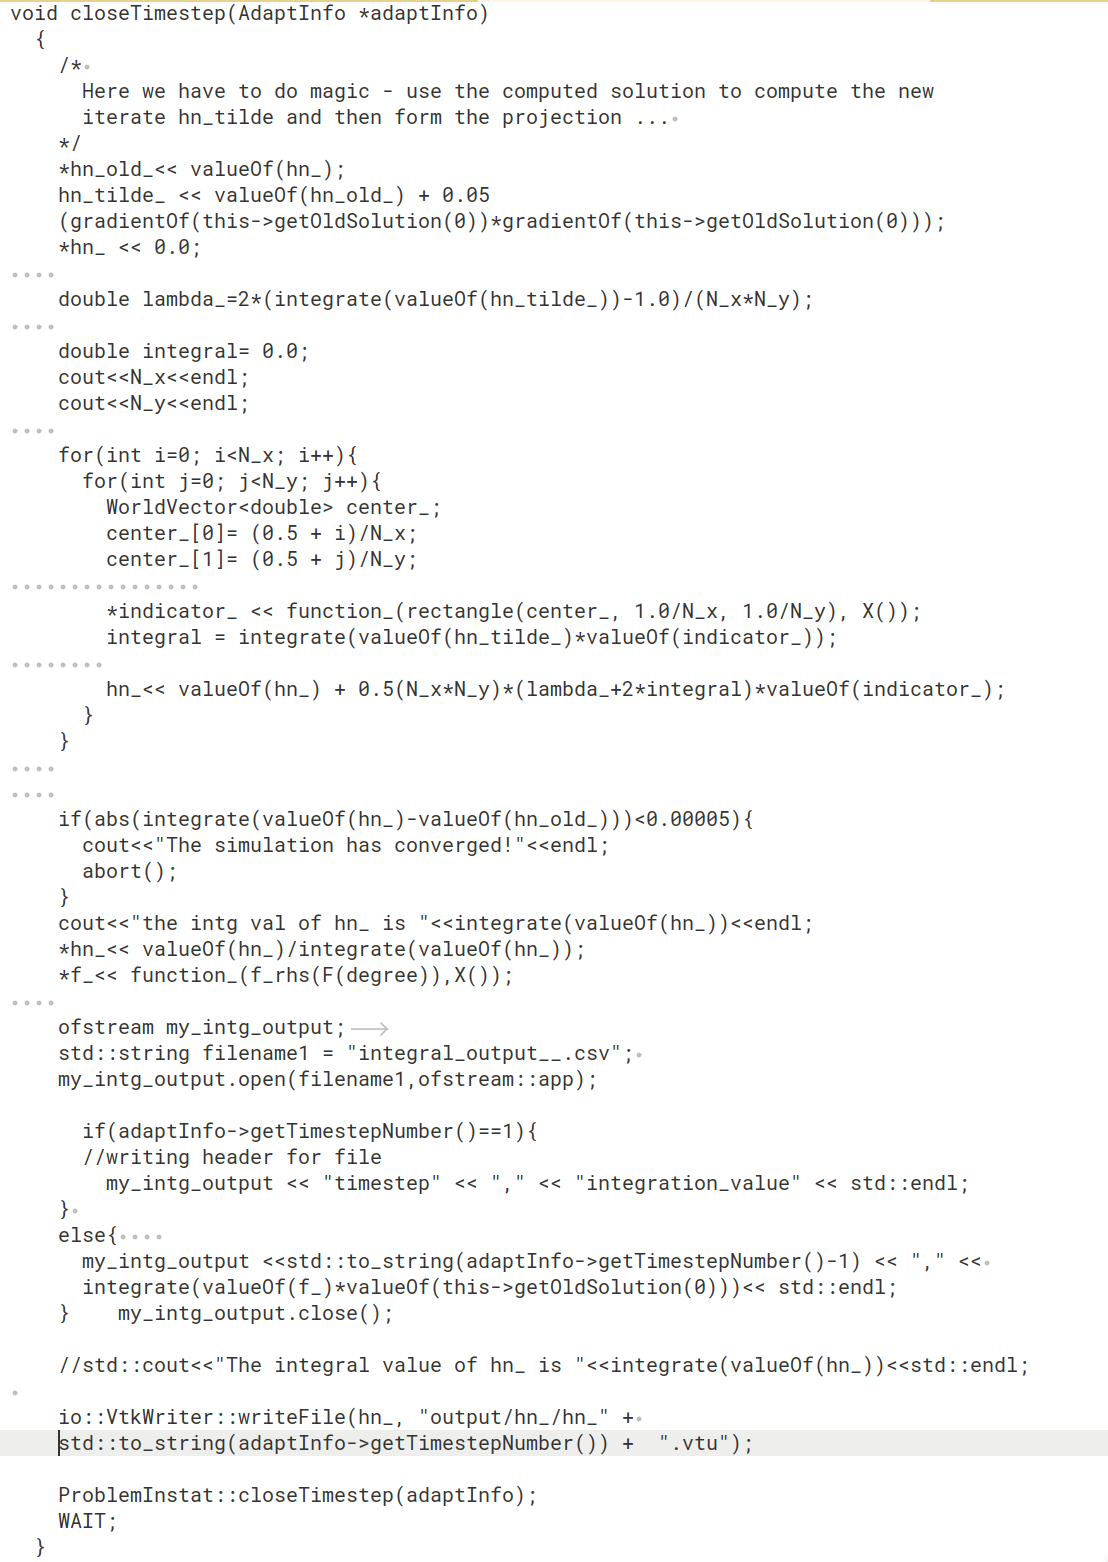
\includegraphics[scale=0.4]{Ctask3.png}


\section{Results} 

We illustrate our method with some different examples. We consider simple stationary problem as an in-stationary one with Dirichlet boundary condition.\\
In Example-1.Figure 6.1(a) we consider force $f = 10*x*y$ with grid spacing $N=N_{x}*N_{y}$= 5*5 = 25.(b) plot of our optimal thickness level.\\
In Example-2.Figure 6.2(a) we consider force $f = -(400x^2 - 20 d )e^-10x^2$ with grid spacing $N=N_{x}*N_{y}$= 10*10 = 100 (b) plot of our optimal thickness level.




\begin{figure}
\centering
\begin{minipage}{.5\textwidth}
  \centering
  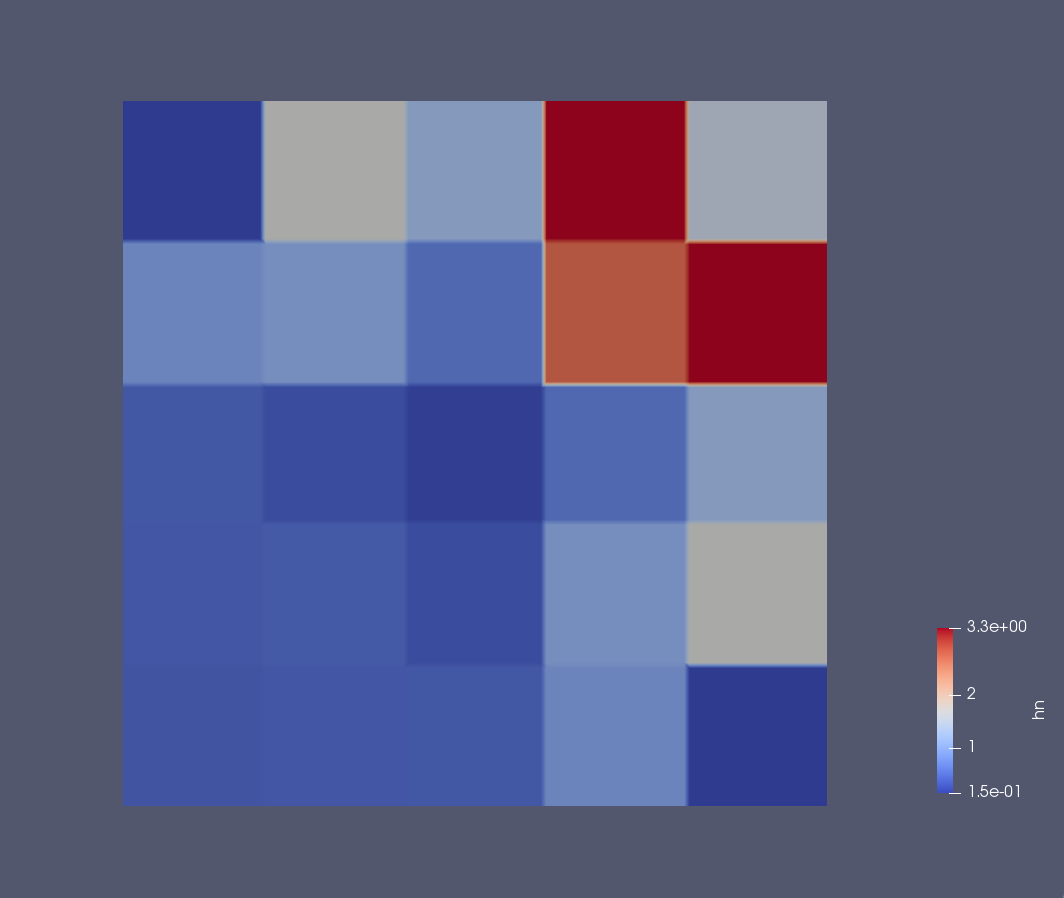
\includegraphics[width=.8\linewidth]{F1.png}
 
  \label{fig:test1}
\end{minipage}%
\begin{minipage}{.5\textwidth}
  \centering
  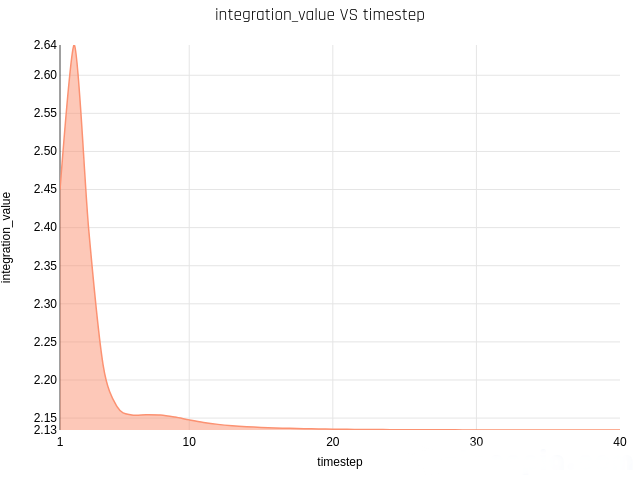
\includegraphics[width=.8\linewidth]{chartF1.png}
  
  \label{fig:test2}
\end{minipage}
\caption{Example-1: left (a) Visualization of thickness, right (b)plot of convergence }
\end{figure}
\begin{figure}
\centering
\begin{minipage}{.5\textwidth}
  \centering
  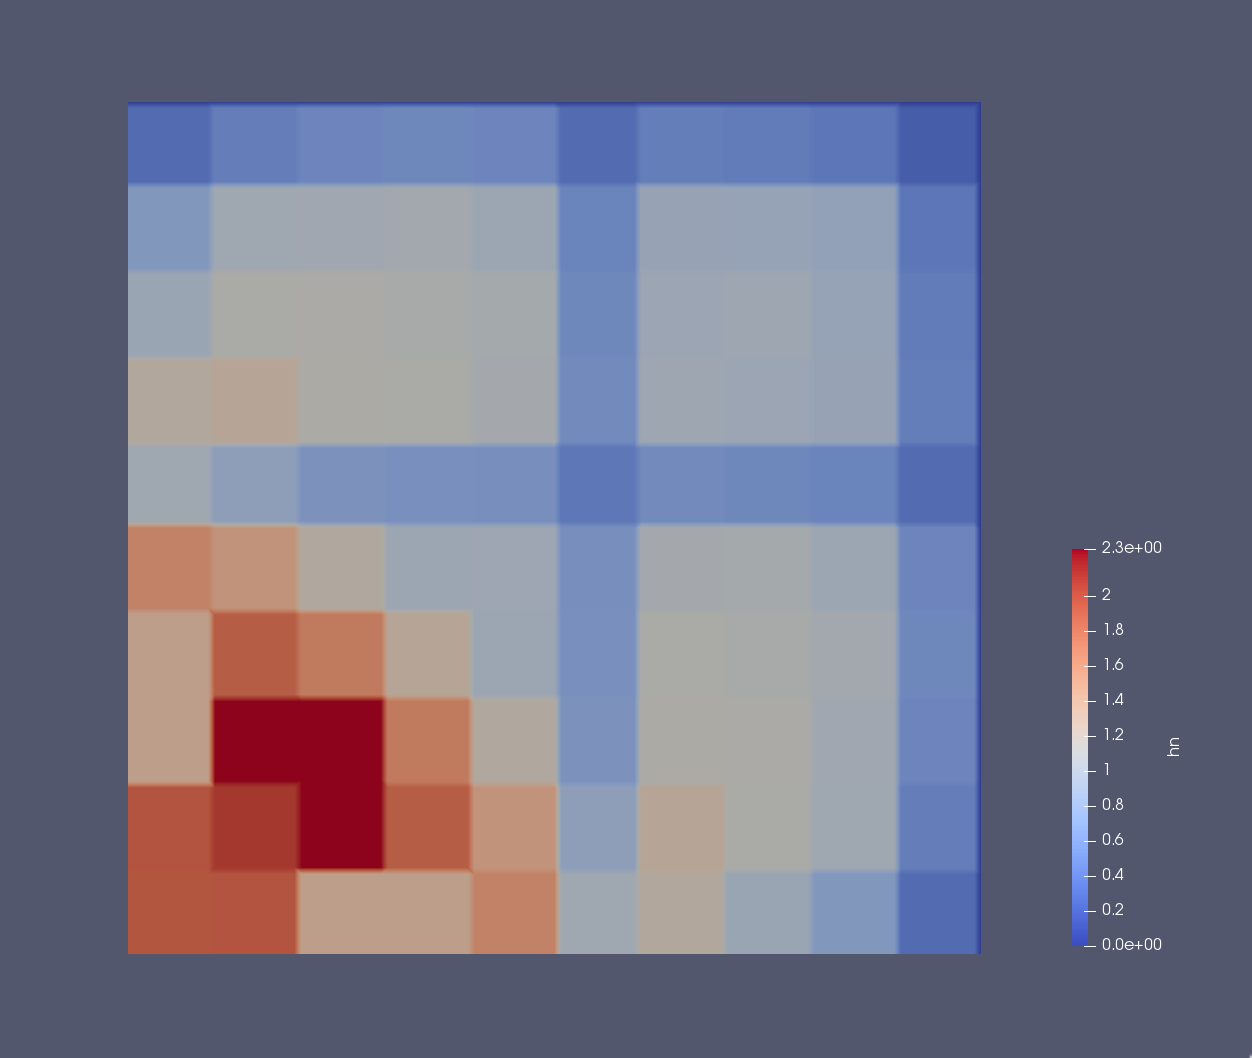
\includegraphics[width=.8\linewidth]{F3.png}
  
  \label{fig:test1}
\end{minipage}%
\begin{minipage}{.5\textwidth}
  \centering
  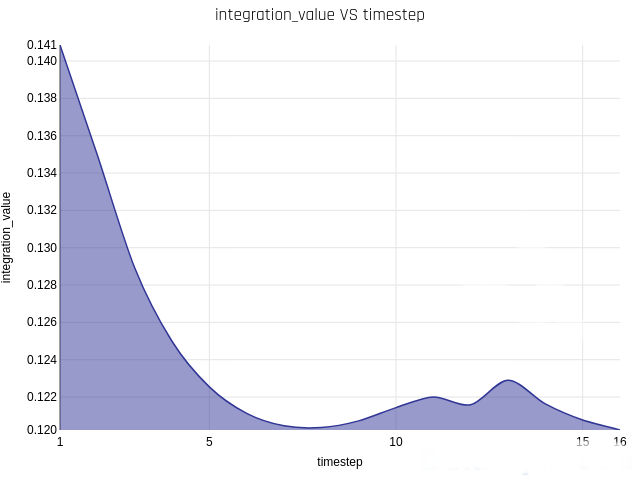
\includegraphics[width=.8\linewidth]{chartF3.png}
  
  \label{fig:test2}
\end{minipage}
\caption{Example-2: left(a) Visualization of thickness, right (b)plot of convergence }
\end{figure}
The result is quite intuitive as the result have a higher thickness in the regions with strong gradients.





\section{Future Scope}
To be honest, there is quite a big room for improvement. Some of the improvements that can be made are.
\begin{description}


 \item
    1. We have just optimized for rigidity. This can be extended to optimize for maximum stress-induced or to achieve a target displacement.
   \item
    2. In this project, we have considered the thickness to be a piece-wise constant. A continuous function in L-infinity is also possible.
     \item
    3. An analysis could be done to see the scaling behavior of the model.
     \item
    4. Adaptive step length could also be used in the gradient method.
     \item
    5. In all our tests, we have initialized our thickness as h=1. We could test different starting points.
     \item
    6. Linearization could be done to improve the computational time.
\end{description}

\section*{Acknowledgment}
This work is done under the guidance of Prof. Dr. Stefan Neukamm, Mario Varga, and Dennis Wenzel. We thank all of you for providing information and resources.

\begin{thebibliography}{9}
\bibitem{latexcompanion} 
Allaire, G., Cavallina, L., Miyake, N., Oka, T., & Yachimura, T. (2019). 
\textit{The homogenization method for topology optimization of structures: old
and new}. 
Interdisciplinary Information Sciences, 25(2), 75-146. (visit
Allaireetal)
 
\bibitem{latexcompanion} 
Braess, Dietrich.  Finite elements. 
\textit{Theory, fast solvers, and applications in-solid mechanics.}. 
 Cambridge University Press, 2007

\end{document}